% This is based on "sig-alternate.tex" V1.9 April 2009
% This file should be compiled with V2.4 of "sig-alternate.cls" April 2009
%
% ---------------------------------------------------------------------------------------------------------------
% This .tex source uses a .bib file (from which the .bbl file % is produced).
% REMEMBER HOWEVER: After having produced the .bbl file, and prior to final
% submission, you *NEED* to 'insert' your .bbl file into your source .tex file
% so as to provide ONE 'self-contained' source file.

\documentclass[10pt,twocolumn]{article}
\usepackage[10pt,nocopyright]{sigmin}
\usepackage[square,comma,numbers,sort&compress]{natbib}
\usepackage{times}
\usepackage{microtype}
\usepackage{color}
\usepackage{graphicx}
\usepackage{listings}
\usepackage{multirow}
\usepackage{url}
\lstset{
  numbers=left, frame=lines, tabsize=2, captionpos=b, numberstyle=\tiny,
  columns=fullflexible, showstringspaces=false, basicstyle=\footnotesize\ttfamily,
  extendedchars=true, breaklines=true
}

\setlength{\columnsep}{.25in}

\begin{document}
\title{Identifying Dating Site Users in 3 Easy Steps}
\author{
  Victor Costan, Daniel Dumitran, Ilia Lebedev,
  Srinivas Devadas and Nickolai Zeldovich \\ \em MIT CSAIL}
\date{}

\maketitle

\begin{abstract}

Users of dating websites expect their profiles on these sites to be anonymous.
We conjecture that many users reuse photos from non-anonymous social networks, such as Facebook, when creating their profiles on dating websites.
We exploit this fact to show a simple method for linking dating profile the profiles.
Specifically, this work introduces a virtually undetectable method for extracting profile information from social networks and dating websites, and a deceptively simple method for matching profile photos across two data sets for the purposes of identifying users on supposedly-anonymous networks.

% QUICK OUTLINE

% Privacy expectation vs reality.
% What to do in order to educate users?

% Technical nugget:

% impersonating users for crawling: chrome debug console to impersonate a user session. Instead of imitating a browser session, we simply instrument one to pro grammatically simulate user input (remote debugging interface for Chromium / Google Chrome).
% Story: sites employ complex countermeasures, while users are not protected from a simple technique. TODO: timing?

% unbreakable in much the same way as screen manipulation, but also have access to DOM structure.

% Secondary:

% Observation that profile photos are taken from a pool of a users ``best'' profile photographs - an often small pool. As a result, a user often reuses the same photographs 
% image similarity, phash. Limitiations. Future work.


\end{abstract}

\section{Introduction}
\label{sec:intro}

Recent years saw a rapid emergence of online dating as an acceptable means of meeting romantic interests.
While a somewhat taboo subject, and a source of some insecurity and hardship for many, dating sites allowed persons equitable access to the dating market regardless of their ability to meet people in their day-to-day lives.
For obvious reasons, online dating carries with it some social stigma and risks, and users prefer to remain anonymous until they explicitly elect to reveal their identity to select individuals.

In fact, privacy and the expectation of anonymity are key to the success of a dating site, as it establishes a relatively safe, on-demand means to access an otherwise risky dating scene.
Users entrust a cache of valuable personal information such as their identity, location, personal preferences, and a wealth of information about personal beliefs.
While the dating sites may do everything in their power to correctly implement their privacy policy and protect the identities of their users, the users themselves must take care to ensure they do not compromise their privacy by revealing identifiable information in a public profile.

De-anonymizing the profiles featured on a dating site is valuable, as it would yield significant amounts of private personal information pertaining to specific individuals.
Some motivations for determining identities of individuals on a dating site may be relatively benign, such as academic or marketing research, a population study, or law enforcement.
There exist legitimate reasons for an individual attempting to ascertain the identity associated with a dating site profile.
Unfortunately, there also exist numerous sinister reasons to de-anonymize dating site profiles, such as stalking, blackmail, public embarrassment, or otherwise offensive or criminal behaviour.

It stands to reason that users' interpretation of a dating site's privacy allows them to delegate some responsibility for maintaining anonymity to the site, enabling a safe environment to share private information.
The site is responsible for correctly implementing their privacy policy, and doing everything in their power to protect the users' identities and information.
Of course no measure is enough to prevent a user from compromising their own privacy by posting identifiable information in their public profile.
Users of dating sites must be educated to understand this in order to avoid being vulnerable to loss of privacy.
In this work, we illustrate that this is indeed a common problem by de-anonymizing a large set of users of a popular dating site.

\subsection{Plan of Attack}
\label{sec:intro_plan_of_attack}

\begin{figure}[hbtp]
  \center{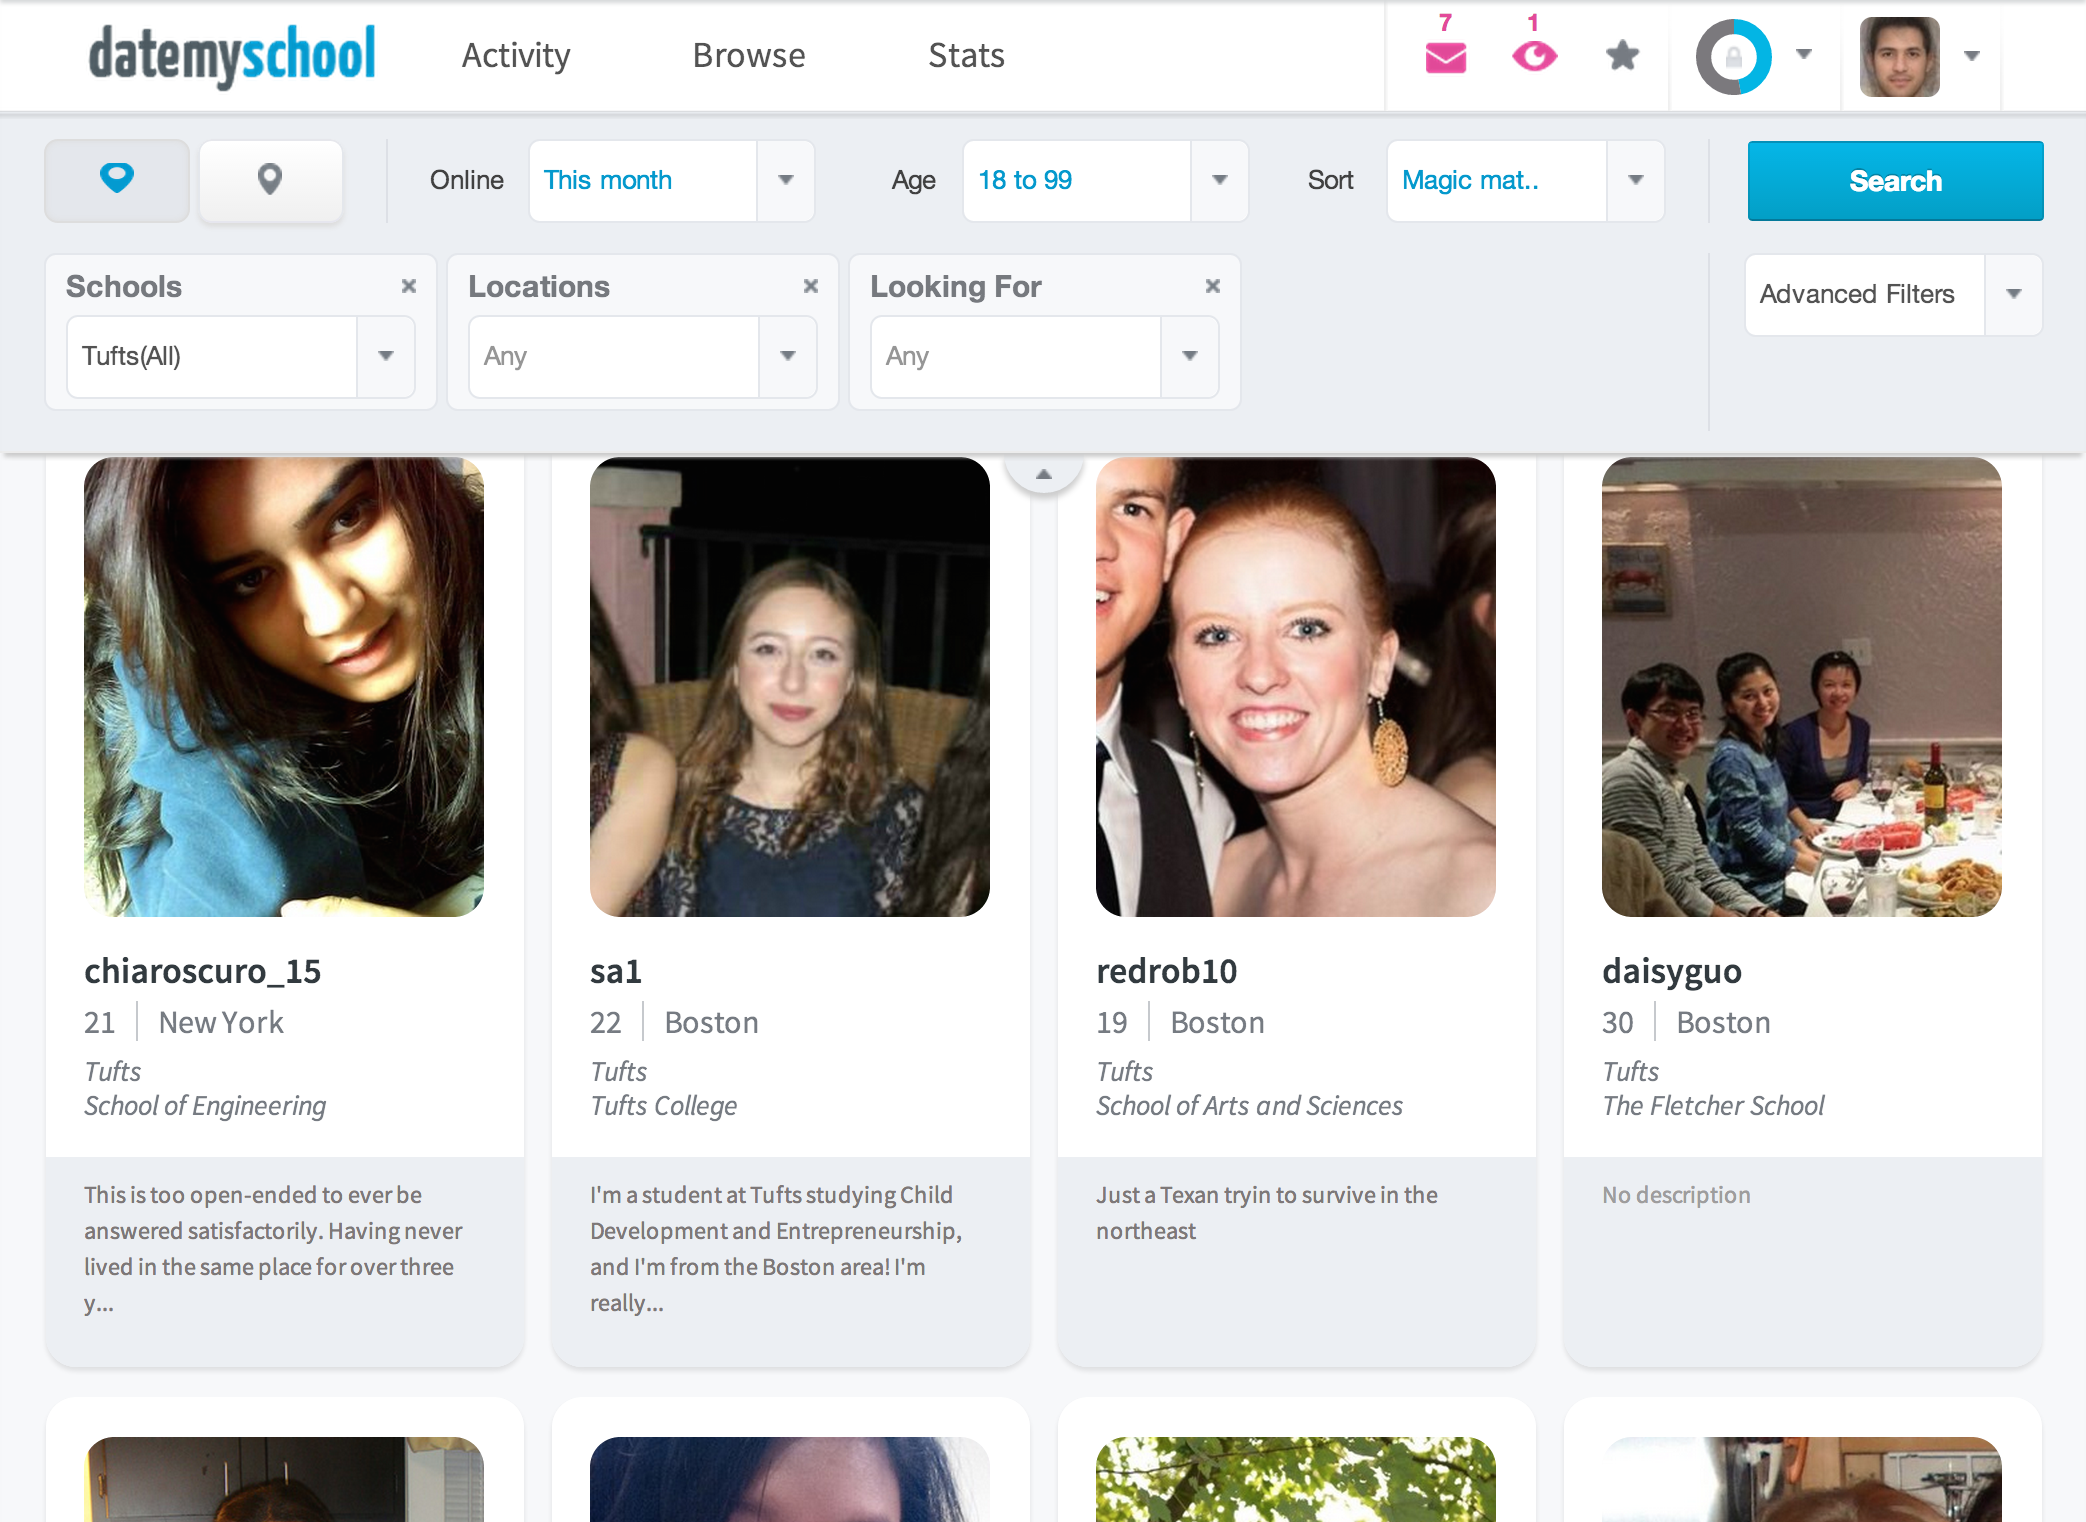
\includegraphics[width=85mm]{figures/dms_search.png}}
  \caption{
    A DateMySchool search for all the female Tufts students.
  }
  \label{fig:dms_search}
\end{figure}

\begin{figure}[hbtp]
  \center{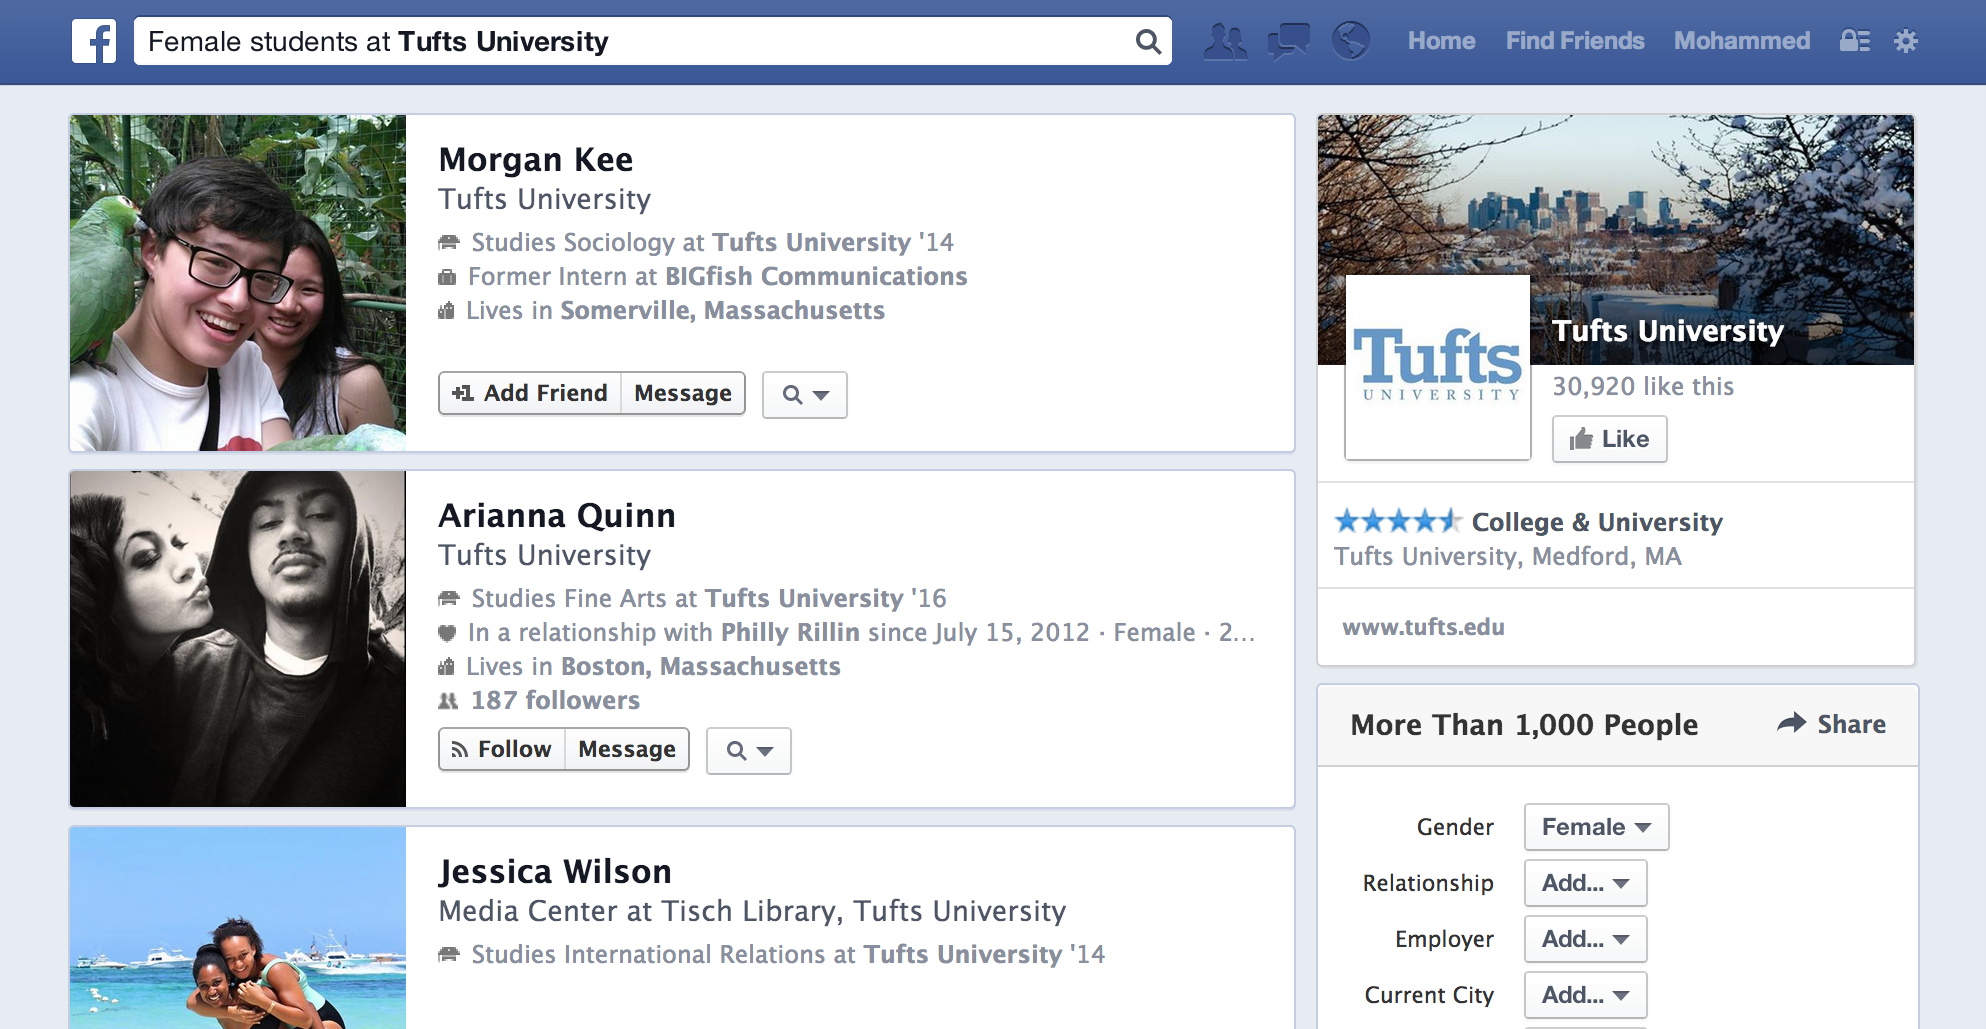
\includegraphics[width=85mm]{figures/fb_search.png}}
  \caption{
    A Facebook search for all the female Tufts students. The results are
    matched against the DateMySchool results for female students.
  }
  \label{fig:fb_search}
\end{figure}

We enumerate a large set of (semi)-public but anonymous profiles featured on the DMS (DateMySchool\cite{dms2014}) site by creating a fictitious account with the dating service and searching for users from Tufts University students, as illustrated in Figure \ref{fig:dms_search}.
This site is popular with college students, as it groups users by school, thereby allowing users to explore the dating market within their academic institution, or with nearby academic institutions, supposedly reducing risk and improving match quality. We take advantage of the school affiliation information in users' profile to reduce the number of Facebook pictures against which we have to match each picture.

We also create a fictitious Facebook\cite{fb2014} account, and use its graph search feature to list all the Tufts University students, as illustrated in \ref{fig:fb_search}. Facebook has a very large user base, and most users list real names, together with vast troves of personal information.
%TODO: does DMS actually require a linked FB account? -- nope, created the facebook way after the DMS account
%In fact, DMS requires a linked Facebook account to sign up, meaning we can expect with a high degree of confidence that each anonymous DMS profile has a non-anonymous Facebook profile.

We then use data set aggregation to correlate the anonymous dating site profiles to non-anonymous Facebook profiles using profile photographs of users as a common feature.
We conjecture that many users will reuse identical photographs on both sites, as they are motivated to select the photos that portray them in the best light.
Since most people have a relatively small set of recent photographs they consider flattering, it would stand to reason that their recent ``good'' photograph used to create a dating site profile would also be featured on Facebook.
Indeed, we found this to be the case with at least TODO\% of the accounts we attempted to de-anonymize.

\section{Related Work}
\label{sec:related}

Online privacy and anonymity has been a hotbed of academic research.
More specifically, dating sites have been shown to be an exciting application with a new cost function and emphasis on user privacy and security~\cite{okws}.


\section{De-Anonymization Of Users of Social Networks}
\label{sec:related_anon}

De-anonymization (also referred to as re-identification) of users on a social network is a high-value research area, and has recieved much attention in recent years, and has been treated increasingly as its own branch of computer science~\cite{reidentification1}.
An growing understanding that a secure, private web is somewhat of an illusion~\cite{webisnotsecure} prompted many users to pay attention to the privacy policy and security measures of the web applications they use~\cite{motivationforanonymity}.
A large body of research, including but not limited to~\cite{deanonsocial1,deanonsocial2,locationprivacy} has been conducted in de-anonymizing users on the internet in order to demystify the illusion of privacy, and better inform future security work.
While profile photos have been identified as a risk to privacy and anonymity~\cite{profilephotos1}, we are not aware of any successful attack on anonymity of a social network via analysis of profile pictures.

Web crawling as a means of data harvesting for large-scale (``big-data'') analysis has been popular with market research, advertising, sentiment analysis, and other applied fields~\cite{crawling1}.
Web application operators seldom derive benefit from web crawling, and may occasionally lose business due to competitors' data gathering, and understandably invest in detecting and curbing large-scale data collection~\cite{limitcrawling1, limitcrawling2, protectidentity1, protectidentity2} and non-human users.

\section{Identifying identical images}
\label{sec:related_images}


Quick identification of similar images is an open research area with many applications ranging from medical imaging to search.~\cite{nearduplicateimage1,nearduplicateimage2}. In this work, we rely on the pHash~\cite{phash} library to implement image comparison, but pHash is unable to align differently cropped images for a robust comparison. There exists a rich body of work for image registration, including ready-to-use solutions~\cite{registration3}.

\section{Design}
\label{sec:design}

In this section, we outline our method for de-anonymizing DMS by aggregating profiles with Facebook data, using profile photos to identify accounts.

\subsection{Impostor Accounts}
\label{sec:design_accounts}

We begin by constructing a fictitious identity and create the accounts necessary to gather information from DMS and Facebook.
The name and photograph are a simple matter of choosing a common name and a profile photograph (using an average-of-faces face). Let \textbf{FU} (``faux-user'') denote the new identity consisting of a fictitious profile photo and a name, as well as some arbitrary profile information, and a made-up birth date.

In order to create a DMS account, \textbf{FU} needs a school-affiliated email (we generated a new \texttt{@mit.edu} address), and a Facebook account - a simple matter of manually filling out a web form and clicking a verification link emailed by Facebook. We are now able to create a fictitious DMS profile for \textbf{FU} by, again, simply filling out a web form.
We do not use existing accounts to avoid compromising our identities, and to avoid unfair advantage such as using a established social network to obtain additional user information.

\subsection{Impersonating Human Users}
\label{sec:design_debug}

We are now able to access both DMS and Facebook using \textbf{FU}'s fictitious account.
Obviously, to de-anonymize DMS profiles on the large scale, we must be able to automate all repeated interaction with the site.
Similarly, we must be able to programmatically extract a large set of Facebook profiles expected to overlap with the extracted DMS profiles.
Creating HTTP sessions within a Python or Ruby script is easy, but is not robust against detection, throttling, and is therefore good approach to extracting large amounts of information from either DMS or Facebook.
While many sophisticated techniques exist to instrument or impersonate human user sessions, ranging from screen manipulation \cite{yeh2009sikuli} to browser impersonation over HTTP requests, we found our approach to be highly effective and very simple.
We use the Chromium remote debugging interface~\cite{chrome-rdb} to instrument a real browser session and programmatically specify user input.
This approach to web crawling uses each site's built-in search functionality in the same way a human user would, meaning the web crawler sessions are virtually impossible to detect at the server.
We effectively impersonate a tablet user, thereby obviating the need to falsify mouse hover data.

The web crawler is coded in as generic a way as possible, as we expect it to be widely applicable to other crawl-able bodies of information online.
For example, a small wrapper over the same the same code base is used to log into both Facebook and DMS, as given in Figure~\ref{fig:login-code}.

\begin{figure*}
\begin{lstlisting}[language=Ruby]
def dms_login(client, email, password)
  client.page_events = true
  client.navigate_to 'https://datemyschool.com'
  client.wait_for type: WebkitRemote::Event::PageLoaded

  login_link = client.dom_root.query_selector '#login-link'
  click_element client, login_link

  login_forms = client.dom_root.query_selector_all 'form[action*="login"]'
  if login_forms.length != 1
    raise 'Login form selector broken or not specific enough'
  end
  login_form = login_forms.first

  email_input = login_form.query_selector 'input[type="text"]'
  input_text client, email_input, email

  password_input = login_form.query_selector 'input[type="password"]'
  input_text client, password_input, password

  submit_button = login_form.query_selector 'input[type="submit"]'
  click_element client, submit_button

  client.wait_for type: WebkitRemote::Event::PageLoaded
  client.page_events = false
  client.clear_all
end

def fb_login(client, email, password)
  client.page_events = true
  client.navigate_to 'https://facebook.com'
  client.wait_for type: WebkitRemote::Event::PageLoaded

  login_forms = client.dom_root.query_selector_all 'form[action*="login"]'
  if login_forms.length != 1
    raise 'Login form selector broken or not specific enough'
  end
  login_form = login_forms.first

  email_input = login_form.query_selector 'input[type="text"]'
  input_text client, email_input, email

  password_input = login_form.query_selector 'input[type="password"]'
  input_text client, password_input, password

  submit_button = login_form.query_selector 'input[type="submit"]'
  click_element client, submit_button

  client.wait_for type: WebkitRemote::Event::PageLoaded
  client.page_events = false
  client.clear_all
end
\end{lstlisting}
\caption{Crawler login code for DMS and Facebook.}
\label{fig:login-code}
\end{figure*}

In crawling DMS, we use the crawler to automatically login, navigate to the search page, and enumerate URLs for all profiles affiliated with a given school. We also download and extract all profile photos affiliated with each account, and store an entry consisting of \texttt{[profile link, photo(s)]} for each DMS user at a given school in an unordered set.

Crawling Facebook is slightly more challenging, as it does not quite allow all members of a school to be enumerated easily. We are, however, able to enumerate all users in the group affiliated with the school - a crude but effective approximation.
Just as with DMS, we extract all profile photographs associated with each account we record.
We store an entry consisting of \texttt{[name, email, photo(s)]} for each Facebook account expected to overlap with the DMS data set we created above.

\subsection{Identifying Profiles}
\label{sec:design_profile}

We now have two (large) data sets of user profiles: anonymous DMS profiles consisting of $D = $\texttt{[profile link, photo(s)]}, and non-anonymous Facebook profiles consisting of $F = $\texttt{[name, email, photo(s)]}.
We expect the ``de-anonymized'' set $U = D \cap F$  (the set of users of both sites) to be significant in size.
To find profiles in $d_u \in D$ and $f_u \in F$ such that $d_u$ and $f_u$ both belong to the same user $u$, we must find a means of correlating anonymous profiles in $D$ with non-anonymous profiles in $F$.

Prior work has relied on text analysis to classify profile authors in order to de-anonymize social networks, but dating sites unfortunately seldom provide a large writing sample.
Unable to rely on text, we instead use other information to correlate profiles.
Fortunately, we found a deceptively simple and accurate means of matching profiles across $D$ and $F$: the profile photos.

We theorize that users rely on a small set of ``good'' photographs for profile photos where they attempt to look their best.
When creating a DMS profile, the users must find a recent high-quality photograph, and we conjecture rely on their Facebook profile photos to select a recent ``good'' image.
As demonstrated in our Results~\ref{sec:results}, the conjecture holds for our initial experiments.
We expect the profile pictures to have been resized and recoded in a lossy way from the original photographs uploaded by the users.
While we cannot simply compare the files, we are nevertheless able to efficiently compare profile photos using the pHash~\cite{phash} library, calculating perceptual hashes of each photo in $D$ and $F$.
Finally, we simply enumerate all pairs $(d_u \in D, f_u \in F)$ such that $d_u$ and $f_u$ have a ``similar'' photo hash (meaning with overwhelming probability an identical profile photo).

\section{Results}
\label{sec:results}

TODO: results

Discuss num of profiles on DMS crawled, challenges, volume of information, crawl times, etc.

Discuss num of profiels on Facebook crawled, challenges, volume of information, crawl times, etc.

Discuss num of profiles de-anonymized. Percept of profiles. 
Discuss challenges, processing times, choice of data structure, algorithms, etc.

Estimate num of profiles vulnerable nation-wide, world-wide on DMS.
Estimate num of profiles vulnerable on other dating sites (OKC, Tinder, Match).

\section{Conclusion}
\label{sec:conclusion}

Sites operating under the promise of anonymity, be it explicit or implied, should do more to educate their users.
Users place some trust in a site when creating a profile in that they delegate the responsibility of maintaining privacy to the site.
These users often fail to understand that the information they share publicly may be enough to de-anonymize their profile, making any measures the site implements to protect their privacy irrelevant. By aggregating multiple data sources, assuming an attacker is able to identify users across data sets, privacy ceases being a simple argument, as the amount of personally identifiable information grows.

In this work, we exploit a common behavior among users (namely, re-use of profile photographs) to de-anonymize a popular dating site (DMS - DateMySchool).
We demonstrate a simple technique to defeat the anonymizing measures of DMS by impersonating a legitimate user using a Chromium remote debugging interface and extracting user data for an entire locale in bulk.
We then use straightforward crawling of a non-anonymous social network (in this work, we use Facebook) to extract public photos and basic identifying information in the same locale.
Conjecturing that many users re-use a small set of photographs for profile pictures, we use the pHash library to implement image comparison and enumerate pairs of accounts on DMS and Facebook that share profile photos.

A simple extension to the flow for creating an anonymous profile would protect users from creating this vulnerability. While DMS is able to go as far as using pHash themselves to ascertain the profile picture is not the same as the one used on Facebook, even a short message warning users of this vulnerability would likely suffice.

\section{Future Work}
\label{sec:related_futurework}

A straightforward extension of this work is to apply the method introduced in this paper to additional schools on DMS, and additional dating sites, such as OK Cupid~\cite{okc}, or Match.com~\cite{match}.

Another direction of future work is to improve the image comparison we rely on to de-anonymize users.
While pHash is very good at finding identical images in different formats and scales, it is not robust to variations in crop and registration (something that many sites allow the users to manipulate).
A robust image comparison metric should be able to normalize image registration. 
\section{Open Source}

Our code is made available in full under the MIT license at the address below:

% TODO(pwnall): move this under csail?
%  - definitely a good idea to snapshot and host on csail

\texttt{https://github.com/pwnall/hibaby}


\setlength{\bibsep}{1pt}
\small
\bibliographystyle{abbrv}
\bibliography{references}

\end{document}
